% -----------------------------------------------
% Template for ISMIR Papers
% 2015 version, based on previous ISMIR templates
% -----------------------------------------------

\documentclass{article}
\usepackage{ismir,amsmath,cite}
\usepackage{graphicx}
\usepackage{color}
\usepackage{amsmath}
\usepackage{amssymb}
\usepackage[]{algorithm2e}
\usepackage{enumitem} 

% Title.
% ------
\title{Paper Template For ISMIR \conferenceyear}


% Single address
% To use with only one author or several with the same address
% ---------------
%\oneauthor
% {Names should be omitted for double-blind reviewing}
% {Affiliations should be omitted for double-blind reviewing}

% Two addresses
% --------------
%\twoauthors
%  {First author} {School \\ Department}
%  {Second author} {Company \\ Address}

% Three addresses
% --------------
\threeauthors
  {First author} {Affiliation1 \\ {\tt author1@ismir.edu}}
  {Second author} {\bf Retain these fake authors in\\\bf submission to preserve the formatting}
  {Third author} {Affiliation3 \\ {\tt author3@ismir.edu}}

% Four addresses
% --------------
%\fourauthors
%  {First author} {Affiliation1 \\ {\tt author1@ismir.edu}}
%  {Second author}{Affiliation2 \\ {\tt author2@ismir.edu}}
%  {Third author} {Affiliation3 \\ {\tt author3@ismir.edu}}
%  {Fourth author} {Affiliation4 \\ {\tt author4@ismir.edu}}

\begin{document}
%
\maketitle
%
\begin{abstract}
The abstract should be placed at the top left column and should contain about 150-200 words.
\end{abstract}
%
\section{Introduction}\label{sec:introduction}

Audio Source separation is a challenging task and fully automatic system is still out of reach, but a number of algorithm involving a human operator are starting to yield satisfactory results. In this context, Non-negative Matrix Factorization (NMF) is a widely used method for source separation. The goal of NMF is to approximate a data matrix $V \in \mathbb{R}_{+}^{n \times m} $ as $V \approx \tilde{V} = WH$ with $W \in \mathbb{R}_{+}^{n \times k}$, $H \in \mathbb{R}_{+}^{k \times m}$ and where $k$ is the rank of factorization \cite{lee99}. In audio signal processing, the input data is usually a Time-Frequency (TF) representation such as a short time Fourier transform (STFT) or a constant-Q transform spectrogram. Blind source separation is a difficult problem and the plain NMF decomposition does not provide satisfying results. To perform a satisfying results, it is necessary to exploit various features that make each sources distinguishable from one another. 
Supervised algorithms in the NMF framework exploit training data or prior information in order to guide the decomposition process. For example information from the scores or from midi signals \cite{EwertM12} can be used to initialize the learning process. The downside of this approach is that it requires well organized prior information that is not always available. Another supervised method consists in performing prior training on specific databases. For example a dictionary matrix $W_{train}$ can be learnt from a big database in order to separate an instrument \cite{jaureguiberry2011adaptation,wudrum}. A common method to build a dictionary for NMF is to perform a decomposition on a large training set. After the convergence, the $W$ matrix from the decomposition is used as the dictionary matrix $W_{train}$ in the separation \cite{jaureguiberry2011adaptation}. Another method is detailed in \cite{wudrum}, a dictionary matrix is created by extracting template spectra from isolated drum samples. The dictionary is then used in a NMF decomposition to perform drum transcription. This method requires minimum tuning from the user. However, the dictionary should match the target instrument for satisfying performances. In this work we will focus on how to build a p supervised algorithms 


\section{Construction of the dictionary}


\subsection{Supervised NMF for source separation}

The NMF model is:
\begin{equation}
V \approx \tilde{V} = WH.
\end{equation}
If $V$ is the power spectrum of a drum signal, The matrix $W$ is a {\em dictionary} or a set of {\em patterns} that codes the frequency information of the data. This dictionary can then be used to extract a specific instrument from a mixture \cite{jaureguiberry2011adaptation,kim2011nonnegative}. However, building a dictionary specific to an instrument and that performs well on a large database is a complicated problem. 


\subsection{Construction of the dictionary}

We decide to use a NMF decomposition for the dictionary. The audio drum signal are from the database \cite{gillet2006enst} and we also used isolated drum sound found on the internet (The dictionary signal used are available on your website). We concatenated $33$ isolated strike on different element of different drum kit to have a wide variety of sounds. The power spectrum of STFT of the drum signal is used as the input for the NMF. We perform an NMF on the test decomposition and we use different rank of factorization to obtain different dictionary.



\section{Page Size}\label{sec:page_size}

The proceedings will be printed on
 \underline{portrait A4-size paper} \underline{(21.0cm x 29.7cm)}.
All material on each page should fit within a rectangle of 17.2cm x 25.2cm,
centered on the page, beginning 2.0cm
from the top of the page and ending with 2.5cm from the bottom.
The left and right margins should be 1.9cm.
The text should be in two 8.2cm columns with a 0.8cm gutter.
All text must be in a two-column format.
Text must be fully justified.

\section{Typeset Text}\label{sec:typeset_text}

\subsection{Normal or Body Text}\label{subsec:body}

Please use a 10pt (point) Times font. Sans-serif or non-proportional fonts
can be used only for special purposes, such as distinguishing source code text.

The first paragraph in each section should not be indented, but all other paragraphs should be.

\subsection{Title and Authors}

The title is 14pt Times, bold, caps, upper case, centered.
Authors' names are omitted when submitting for double-blind reviewing.
The following is for making a camera-ready version.
Authors' names are centered.
The lead author's name is to be listed first (left-most), and the co-authors' names after.
If the addresses for all authors are the same, include the address only once, centered.
If the authors have different addresses, put the addresses, evenly spaced, under each authors' name.

\subsection{First Page Copyright Notice}

Please include the copyright notice exactly as it appears here in the lower left-hand corner of the page.
It is set in 8pt Times.

\subsection{Page Numbering, Headers and Footers}

Do not include headers, footers or page numbers in your submission.
These will be added when the publications are assembled.

\section{First Level Headings}

First level headings are in Times 10pt bold,
centered with 1 line of space above the section head, and 1/2 space below it.
For a section header immediately followed by a subsection header, the space should be merged.

\subsection{Second Level Headings}

Second level headings are in Times 10pt bold, flush left,
with 1 line of space above the section head, and 1/2 space below it.
The first letter of each significant word is capitalized.

\subsubsection{Third and Further Level Headings}

Third level headings are in Times 10pt italic, flush left,
with 1/2 line of space above the section head, and 1/2 space below it.
The first letter of each significant word is capitalized.

Using more than three levels of headings is highly discouraged.

\section{Footnotes and Figures}

\subsection{Footnotes}

Indicate footnotes with a number in the text.\footnote{This is a footnote.}
Use 8pt type for footnotes. Place the footnotes at the bottom of the page on which they appear.
Precede the footnote with a 0.5pt horizontal rule.

\subsection{Figures, Tables and Captions}

All artwork must be centered, neat, clean, and legible.
All lines should be very dark for purposes of reproduction and art work should not be hand-drawn.
The proceedings are not in color, and therefore all figures must make sense in black-and-white form.
Figure and table numbers and captions always appear below the figure.
Leave 1 line space between the figure or table and the caption.
Each figure or table is numbered consecutively. Captions should be Times 10pt.
Place tables/figures in text as close to the reference as possible.
References to tables and figures should be capitalized, for example:
see \figref{fig:example} and \tabref{tab:example}.
Figures and tables may extend across both columns to a maximum width of 17.2cm.

\begin{table}
 \begin{center}
 \begin{tabular}{|l|l|}
  \hline
  String value & Numeric value \\
  \hline
  Hello ISMIR  & \conferenceyear \\
  \hline
 \end{tabular}
\end{center}
 \caption{Table captions should be placed below the table.}
 \label{tab:example}
\end{table}

\begin{figure}
 \centerline{\framebox{
 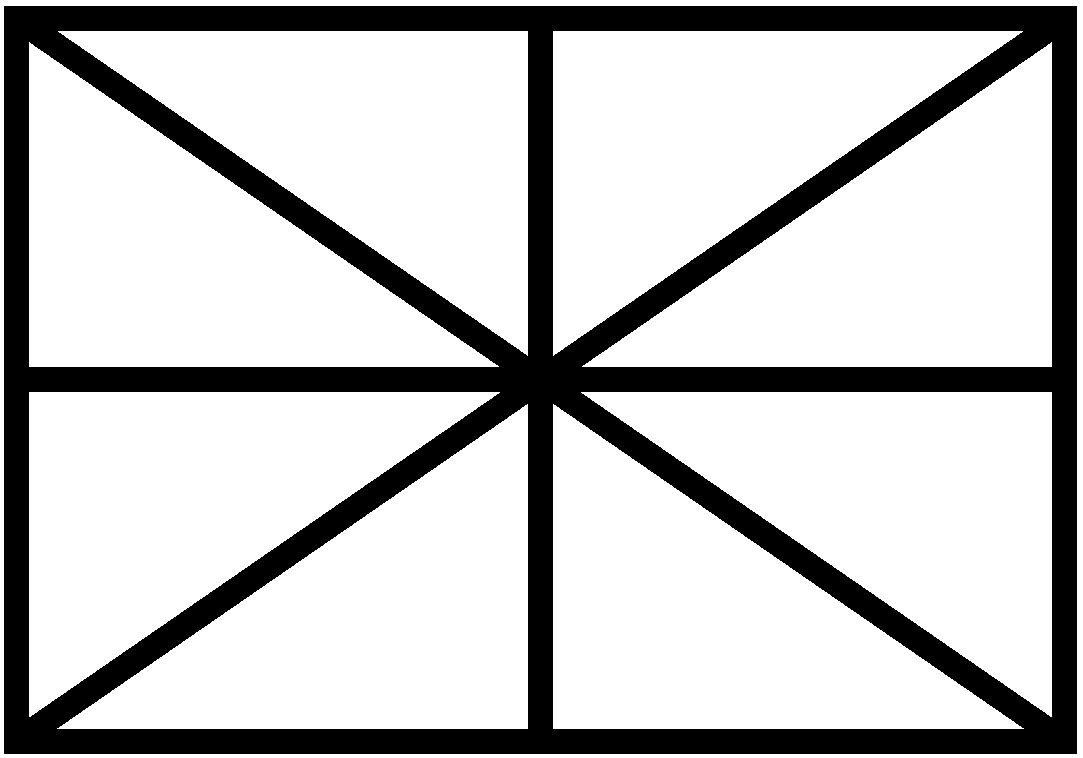
\includegraphics[width=\columnwidth]{figure.png}}}
 \caption{Figure captions should be placed below the figure.}
 \label{fig:example}
\end{figure}

\section{Equations}

Equations should be placed on separate lines and numbered.
The number should be on the right side, in parentheses, as in \eqnref{relativity}.

\begin{equation}\label{relativity}
E=mc^{2}
\end{equation}

\section{Citations}

\bibliographystyle{IEEEtran}

% For bibtex users:
\bibliography{reference}

% For non bibtex users:
%\begin{thebibliography}{citations}
%
%\bibitem {Author:00}
%E. Author.
%``The Title of the Conference Paper,''
%{\it Proceedings of the International Symposium
%on Music Information Retrieval}, pp.~000--111, 2000.
%
%\bibitem{Someone:10}
%A. Someone, B. Someone, and C. Someone.
%``The Title of the Journal Paper,''
%{\it Journal of New Music Research},
%Vol.~A, No.~B, pp.~111--222, 2010.
%
%\bibitem{Someone:04} X. Someone and Y. Someone. {\it Title of the Book},
%    Editorial Acme, Porto, 2012.
%
%\end{thebibliography}

\end{document}
